% Shared vector grammar. Generated figure TeX files inline this source.
\documentclass[tikz,border=4mm,12pt]{standalone}
\usepackage[UTF8,fontset=fandol]{ctex}
\usepackage{amsmath,amssymb,bm}
\renewcommand{\familydefault}{\sfdefault}
\hyphenpenalty=10000
\exhyphenpenalty=10000
\usetikzlibrary{arrows.meta,backgrounds,calc}
\definecolor{Ink}{HTML}{273648}
\definecolor{Muted}{HTML}{607086}
\definecolor{Ctx}{HTML}{85898F}
\definecolor{Qst}{HTML}{4F8FA5}
\definecolor{Opt}{HTML}{5A9A6E}
\definecolor{Gen}{HTML}{B89A5E}
\definecolor{Hid}{HTML}{8A74B5}
\definecolor{Wgt}{HTML}{E0904F}
\definecolor{Lgt}{HTML}{C95B5B}
\definecolor{Idx}{HTML}{7E8B9B}
\definecolor{Msk}{HTML}{3F5A78}
\newcommand{\Unit}{0.30}
\newcommand{\Offset}{0.12}
\newcommand{\BinarySupport}{0}
\newcounter{texture}
\tikzset{
 flow/.style={-{Latex[length=2mm,width=1.5mm]},draw=Ink!75,line width=.65pt},
 tensorlabel/.style={font=\small,text=Ink,align=center,inner sep=0pt},
 tenshape/.style={font=\scriptsize,text=Muted,align=center,inner sep=0pt},
 stage/.style={font=\small\bfseries,text=Muted,align=left,anchor=west},
 operation/.style={draw=Ink!25,fill=white,rounded corners=2pt,align=center,
  font=\small,text=Ink,inner sep=5pt,line width=.5pt},
}
% The last two axes define a matrix face. Leading axes use offset sheets.
% Every symbolic dimension maps to the same cell count throughout the set.
\newcommand{\Tensor}[9]{%
 \stepcounter{texture}
 \pgfmathsetmacro{\ww}{#5*\Unit}
 \pgfmathsetmacro{\hh}{#4*\Unit}
 \pgfmathsetmacro{\xx}{#2-\ww/2}
 \pgfmathsetmacro{\yy}{#3-\hh/2}
 \ifnum#7>0
  \foreach \s in {#7,...,1}{
   \path[draw=#6!40,fill=white,line width=.45pt,rounded corners=.7pt]
    ({\xx+\s*\Offset},{\yy+\s*\Offset}) rectangle ++(\ww,\hh);}
 \fi
 \foreach \r in {1,...,#4}{\foreach \c in {1,...,#5}{
  \ifnum\BinarySupport>0
   \pgfmathtruncatemacro{\level}{\BinarySupport==1?(\c>3-\r?75:0):(\BinarySupport==2?(\c<=4-\r?75:0):(\c<=\r?75:0))}
  \else
   \pgfmathtruncatemacro{\tone}{mod(\r*13+\c*7+\arabic{texture}*11,7)}
   \pgfmathtruncatemacro{\level}{\tone<3?30:(\tone<6?55:80)}
  \fi
  \path[fill=#6!\level,rounded corners=.5pt]
   ({\xx+(\c-1)*\Unit+.021},{\yy+\hh-\r*\Unit+.021})
    rectangle ++({\Unit-.042},{\Unit-.042});}}
 \ifnum\BinarySupport>0
  \path[draw=Msk!35,line width=.4pt] (\xx,\yy) rectangle ++(\ww,\hh);
 \fi
 \coordinate (#1-w) at (\xx,#3);
 \coordinate (#1-e) at ({\xx+\ww+#7*\Offset},#3);
 \node[tensorlabel] at (#2,{\yy-.28}) {$#8$};
 \node[tenshape] at (#2,{\yy-.63}) {$#9$};
}
% Exact binary support; row i is a query and column j a key.
\newcommand{\Support}[5]{%
 \foreach \i in {1,...,#4}{\foreach \j in {1,...,#4}{
  \pgfmathtruncatemacro{\on}{#5}
  \ifnum\on>0
   \path[fill=Msk!65,rounded corners=.4pt]
    ({#2+(\j-1)*\Unit+.021},{#3-\i*\Unit+.021})
     rectangle ++({\Unit-.042},{\Unit-.042});
  \fi}}
 \path[draw=Ink!35,line width=.4pt] (#2,#3) rectangle ++({#4*\Unit},{-#4*\Unit});
}
\newcommand{\Meaning}[7]{%
 \node[anchor=north west,fill=Ink!4,rounded corners=3pt,inner sep=9pt,
  text width=#3cm-18pt,align=left,font=\small] (meaning) at (#1,#2) {
  \begin{tabular}{@{}p{1.8cm}@{\hspace{7pt}}p{\dimexpr #3cm-2.8cm\relax}@{}}
   \textbf{#4} & \raggedright #5\tabularnewline[6pt]
   \textbf{#6} & \raggedright #7\tabularnewline
  \end{tabular}};
}

\begin{document}
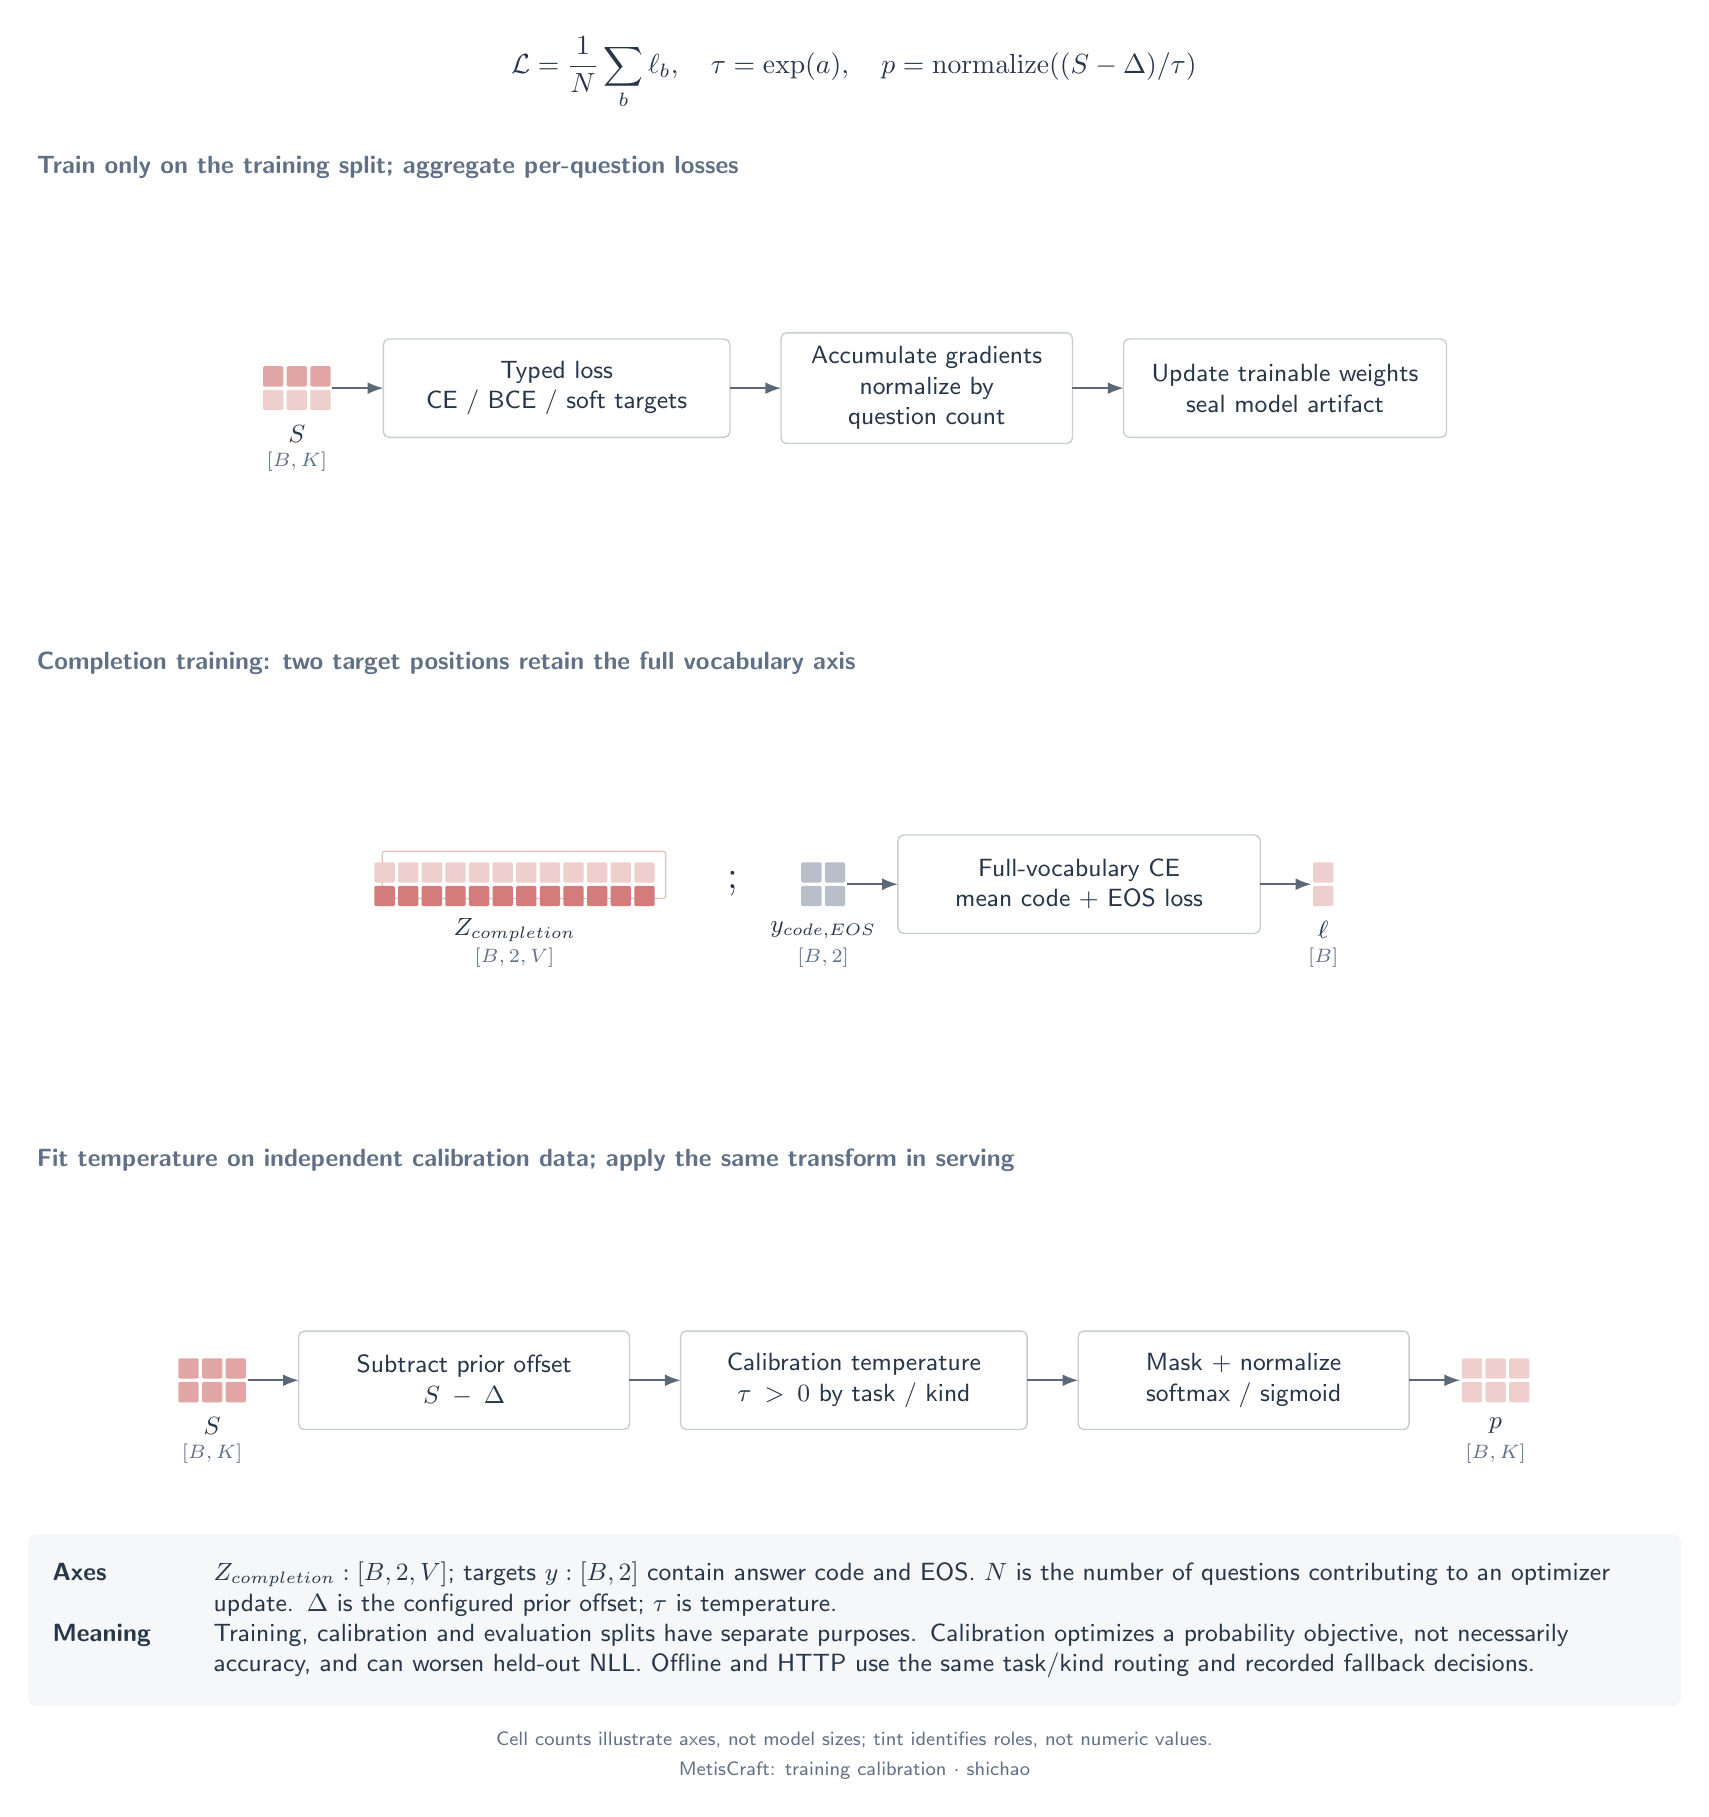
\begin{tikzpicture}[x=1cm,y=1cm,text=Ink]
\node[font=\normalsize,align=center] at (10.500,4.0) {$\displaystyle \mathcal L=\frac{1}{N}\sum_b\ell_b,\quad \tau=\exp(a),\quad p=\operatorname{normalize}((S-\Delta)/\tau)$};
\node[stage] at (0,2.800) {Train only on the training split; aggregate per-question losses};
\renewcommand{\BinarySupport}{0}
\Tensor{r0n0}{3.425}{-0.000}{2}{3}{Lgt}{0}{S}{[B,K]}
\node[operation,minimum width=4.400cm,minimum height=1.250cm,text width=4.050cm] (r0n1) at (6.725,-0.000) {Typed loss\\CE / BCE / soft targets};
\coordinate (r0n1-w) at (4.525,-0.000);\coordinate (r0n1-e) at (8.925,-0.000);
\draw[flow] (r0n0-e) -- (r0n1-w);
\node[operation,minimum width=3.700cm,minimum height=1.250cm,text width=3.350cm] (r0n2) at (11.425,-0.000) {Accumulate gradients\\normalize by question count};
\coordinate (r0n2-w) at (9.575,-0.000);\coordinate (r0n2-e) at (13.275,-0.000);
\draw[flow] (r0n1-e) -- (r0n2-w);
\node[operation,minimum width=4.100cm,minimum height=1.250cm,text width=3.750cm] (r0n3) at (15.975,-0.000) {Update trainable weights\\seal model artifact};
\coordinate (r0n3-w) at (13.925,-0.000);\coordinate (r0n3-e) at (18.025,-0.000);
\draw[flow] (r0n2-e) -- (r0n3-w);
\node[stage] at (0,-3.500) {Completion training: two target positions retain the full vocabulary axis};
\renewcommand{\BinarySupport}{0}
\Tensor{r1n0}{6.190}{-6.300}{2}{12}{Lgt}{1}{Z_{completion}}{[B,2,V]}
\node[font=\Large] (r1n1) at (8.960,-6.300) {$ ; $};
\coordinate (r1n1-w) at (8.760,-6.300);\coordinate (r1n1-e) at (9.160,-6.300);
\renewcommand{\BinarySupport}{0}
\Tensor{r1n2}{10.110}{-6.300}{2}{2}{Idx}{0}{y_{code,EOS}}{[B,2]}
\node[operation,minimum width=4.600cm,minimum height=1.250cm,text width=4.250cm] (r1n3) at (13.360,-6.300) {Full-vocabulary CE\\mean code + EOS loss};
\coordinate (r1n3-w) at (11.060,-6.300);\coordinate (r1n3-e) at (15.660,-6.300);
\draw[flow] (r1n2-e) -- (r1n3-w);
\renewcommand{\BinarySupport}{0}
\Tensor{r1n4}{16.460}{-6.300}{2}{1}{Lgt}{0}{\ell}{[B]}
\draw[flow] (r1n3-e) -- (r1n4-w);
\node[stage] at (0,-9.800) {Fit temperature on independent calibration data; apply the same transform in serving};
\renewcommand{\BinarySupport}{0}
\Tensor{r2n0}{2.350}{-12.600}{2}{3}{Lgt}{0}{S}{[B,K]}
\node[operation,minimum width=4.200cm,minimum height=1.250cm,text width=3.850cm] (r2n1) at (5.550,-12.600) {Subtract prior offset\\$S-\Delta$};
\coordinate (r2n1-w) at (3.450,-12.600);\coordinate (r2n1-e) at (7.650,-12.600);
\draw[flow] (r2n0-e) -- (r2n1-w);
\node[operation,minimum width=4.400cm,minimum height=1.250cm,text width=4.050cm] (r2n2) at (10.500,-12.600) {Calibration temperature\\$\tau>0$ by task / kind};
\coordinate (r2n2-w) at (8.300,-12.600);\coordinate (r2n2-e) at (12.700,-12.600);
\draw[flow] (r2n1-e) -- (r2n2-w);
\node[operation,minimum width=4.200cm,minimum height=1.250cm,text width=3.850cm] (r2n3) at (15.450,-12.600) {Mask + normalize\\softmax / sigmoid};
\coordinate (r2n3-w) at (13.350,-12.600);\coordinate (r2n3-e) at (17.550,-12.600);
\draw[flow] (r2n2-e) -- (r2n3-w);
\renewcommand{\BinarySupport}{0}
\Tensor{r2n4}{18.650}{-12.600}{2}{3}{Lgt}{0}{p}{[B,K]}
\draw[flow] (r2n3-e) -- (r2n4-w);
\Meaning{0}{-14.550}{21.000}{Axes}{$Z_{completion}:[B,2,V]$; targets $y:[B,2]$ contain answer code and EOS. $N$ is the number of questions contributing to an optimizer update. $\Delta$ is the configured prior offset; $\tau$ is temperature.}{Meaning}{Training, calibration and evaluation splits have separate purposes. Calibration optimizes a probability objective, not necessarily accuracy, and can worsen held-out NLL. Offline and HTTP use the same task/kind routing and recorded fallback decisions.}
\node[font=\scriptsize,text=Muted,anchor=north,align=center] at ($(meaning.south)+(0,-.2)$) {Cell counts illustrate axes, not model sizes; tint identifies roles, not numeric values.\\[3pt]MetisCraft: training calibration $\cdot$ shichao};
\end{tikzpicture}
\end{document}
